\chapter{Kliensközeli komponensek implementációja}

A következőkben részletezem a klienseket kiszolgáló infrastrukturális komponensek konfigurációját, valamint a legfelső megjelenítési réteg szoftveres komponenseinek implementációját. A forgalom először a CDN-nel ütközik, amelyen keresztül lesznek elérhetőek a~statikus weboldal erőforrásai, valamint a média-erőforrások csatornái.

\section{A CDN és a hozzácsatolt erőforrások}

A CDN és az ahhoz tartozó erőforrások jelentik az első belépési pontját egy a rendszerhez intézett kérésnek. A rendszer és a CDN -- azaz a CloudFront-disztribúció -- számára a~\verb|stream.trisz.hu| doménnevet rendeltem, amelyet a saját \verb|trisz.hu| doménem aldoménjeként jegyeztem be a~Route 53 szolgáltatásban egy külön DNS zónaként. A böngészőből, azaz kívülről indított kérések minden esetben a DNS feloldásával kezdődnek, a~Route 53 névszervereire oldódik fel, ezzel szerzi meg a kliens az IP-jét a CloudFront edge szerverfarmjának. A CloudFront-disztribúcióknak különleges CNAME rekordjaik vannak, biztosítják hogy a kliens a legközelebbi edge szerverfarmhoz csatlakozhasson, a konkrét működést az AWS elrejti a háztető alatt előlünk. A biztonságos, HTTPS-alapú szerver--kliens kommunikációt a CloudFront-disztribúcióhoz tartozó SSL-tanúsítvánnyal biztosítja a rendszer. A tanúsítványt az AWS Certificate Manager szolgáltatásban generáltam és kezeltem, amely automatikusan megújítja a lejáró tanúsítványokat, amennyiben a doménhez tartozó DNS-zónát a Route 53 szolgáltatásban -- azaz az AWS szolgáltatásában kezeljük.

A CloudFront-disztribúcióhoz hozzácsatoltam egy WAF ACL-t, amely a webalkalmazás szintű tűzfal szerepét tölti be. Minden kérést ez a Layer 7 rétegbeli logika szűri meg. Mivel nem volt élő forgalomra készítve az alkalmazás, így egy egyszerű AWS menedzselte szabályt tettem csak rá a WAF-ra demonstrációképp, amely megvizsgálja a kérést, hogy tartalmaz-e SQL injection támadást vagy egyéb megszokott webalkalmazásokra jellemző ilyen jellegű támadást (pl.: ismert kihasználható URI`|útvonalak, Java webalkalmazásokra jellemző exploitok) -- a szabálycsoportot név szerint \verb|AWSManagedRulesKnownBadInputsRuleSet| név alatt tartja számon az AWS WAF.

Az edge-en kerül kiértékelésre a kapott kérés útvonala (angolul \emph{path}) alapján az, hogy melyik origin felé kell továbbítsa a disztribúció a kérést.

\begin{figure}[h]
  \centering
  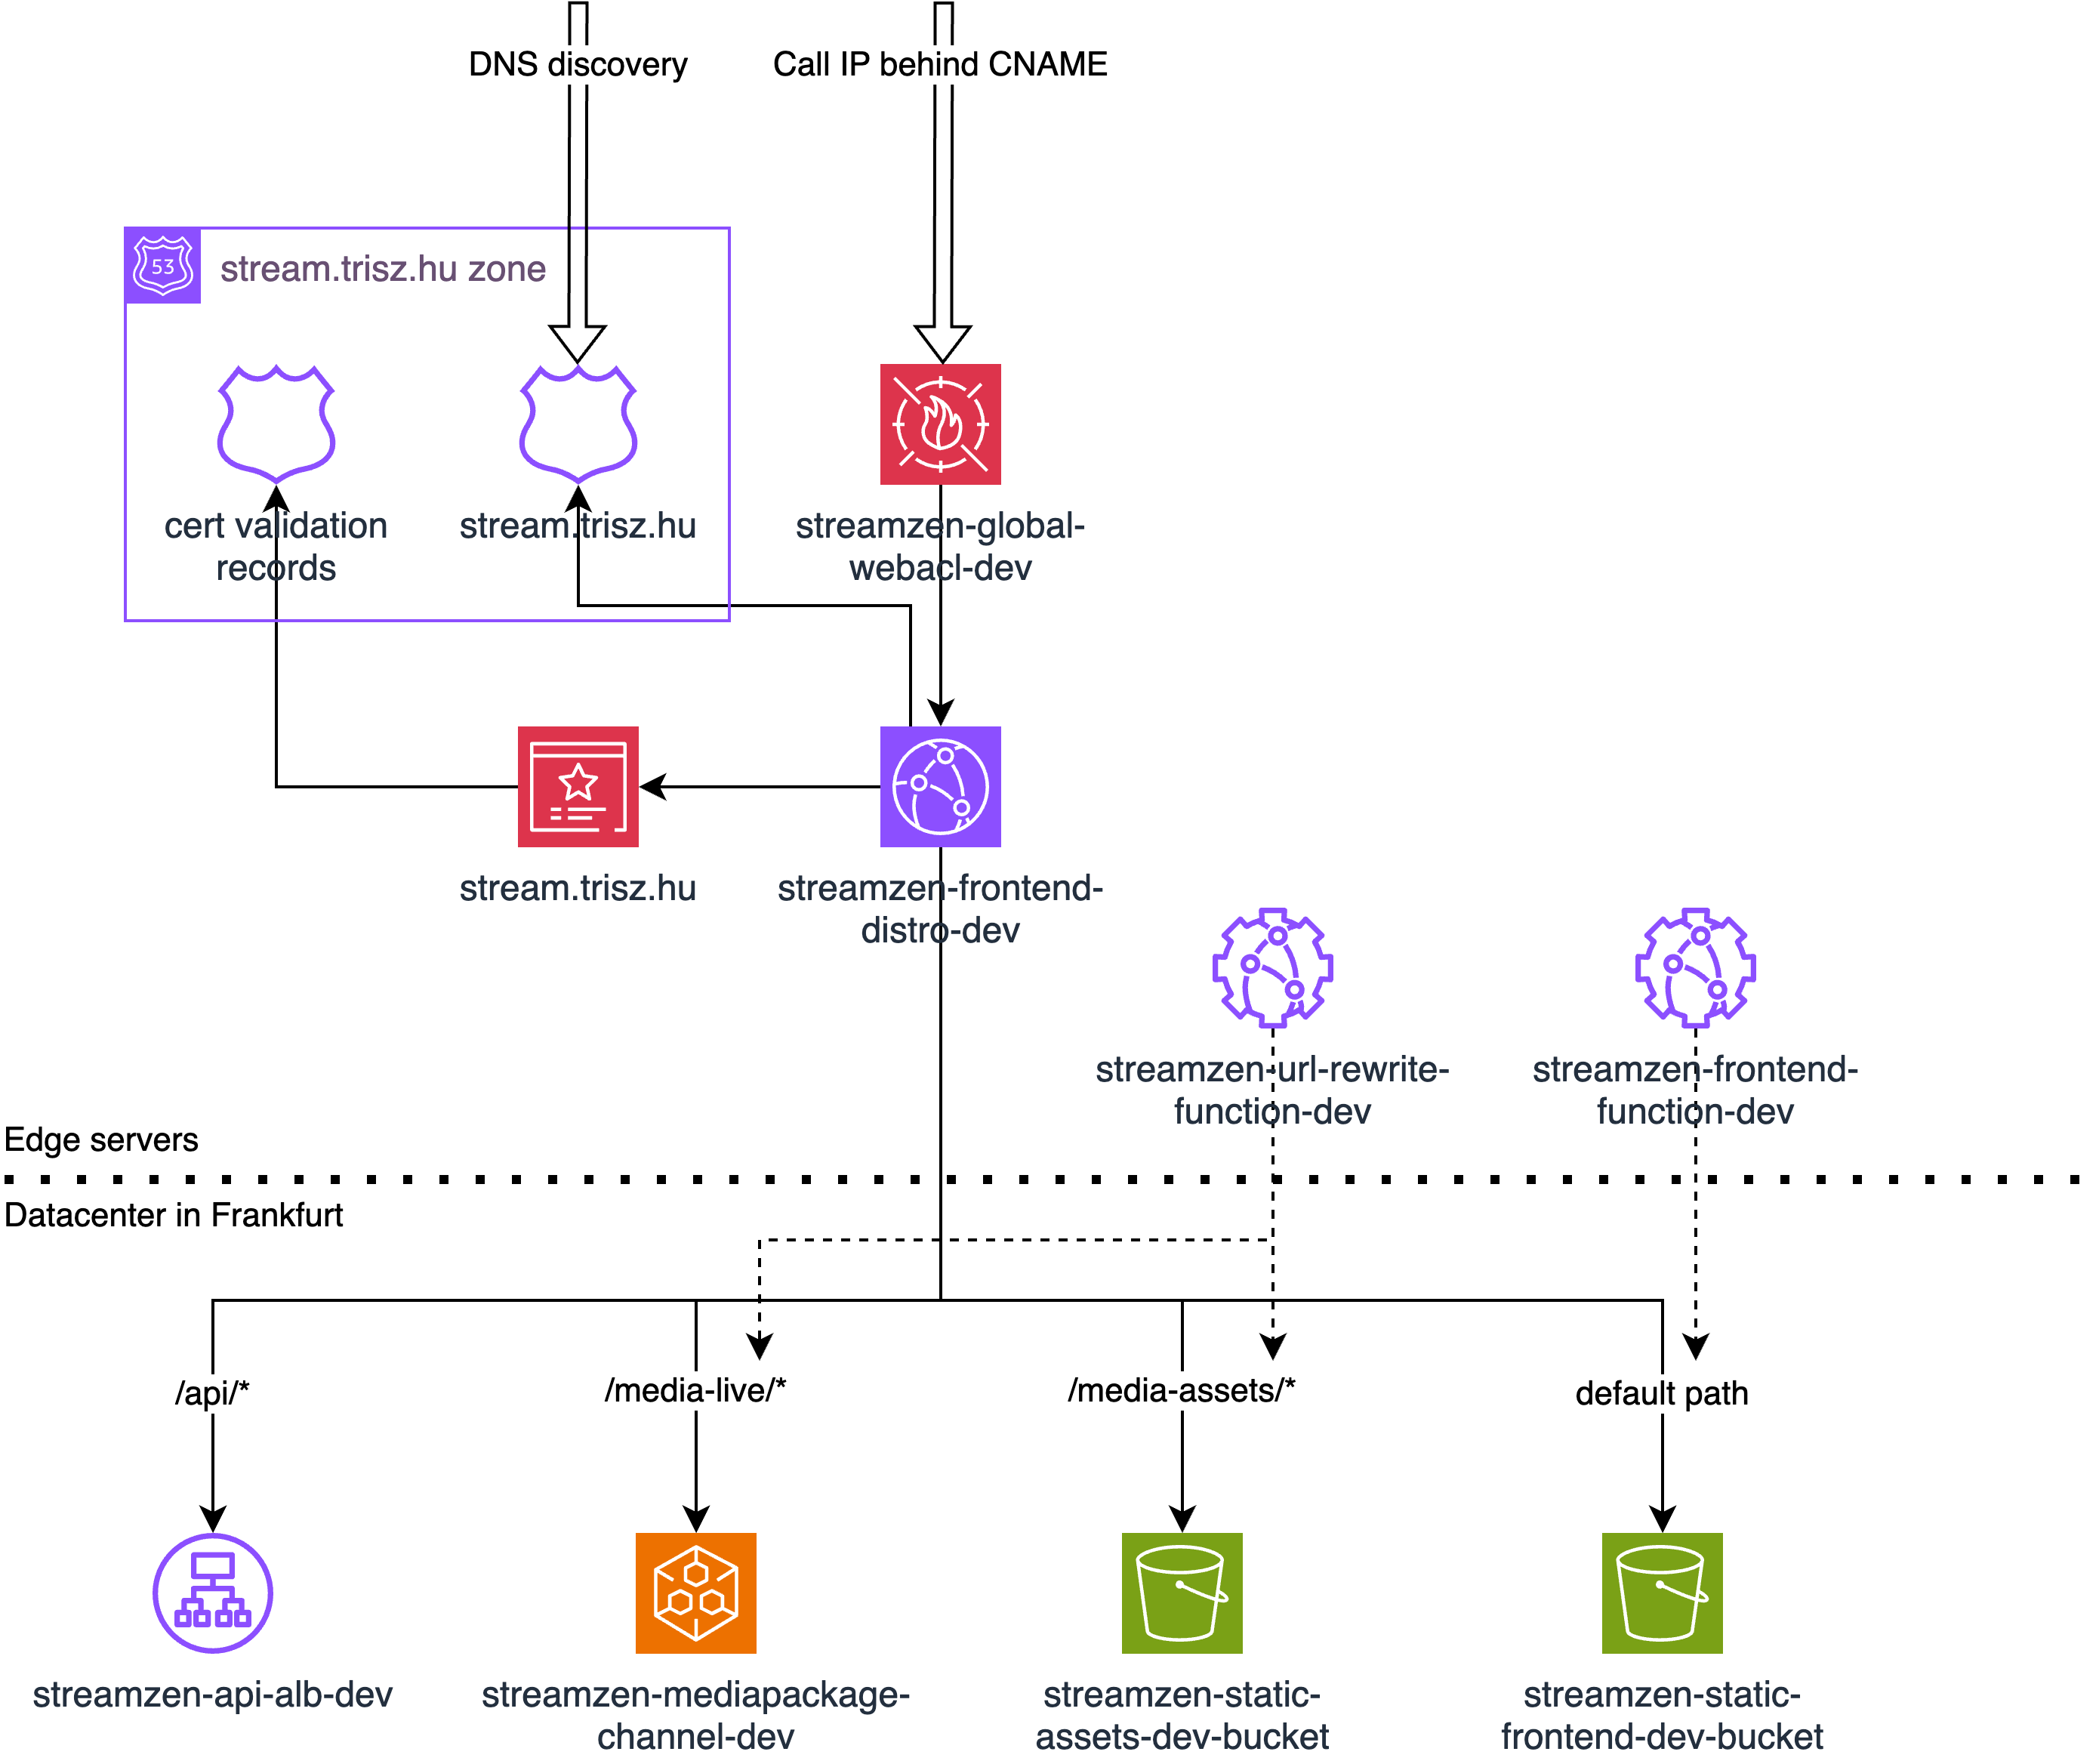
\includegraphics[width=150mm, keepaspectratio]{figures/dipterv_client.png}
  \caption{A kliensoldali architektúra részletesebben.}
  \label{fig:client}
\end{figure}

\Az+\refstruc{fig:client} adatközpont (angolul \emph{datacenter}) felőli oldalán láthatóak a nyilak végén, hogy milyen útvonalak alapján kerül a kérés melyik originhez. A kiértékelés során a disztribúció figyelembe veszi a szabályok sorrendjét, az szabályokban definiált útvonalmintákra mintaillesztés történik, és ha kapott útvonal illeszkedik a sorban következő mintára, ott véget és a kiértékelés. A disztribúcióhoz tartozó originok közül a legfontosabb a statikus weboldal, amely az S3-vödörben található, ez lett az alapértelmezett útvonal, ahova a kérések mennek, amennyiben egyik előbbi útvonalmintára se illeszkedik a kérésben található útvonal.

A CloudFront biztosítja, hogy kis számításigényű logikát tudjuk még az edge rétegében futtatni a kéréseken, erre CloudFront Function-függvényeket alkalmaztam a~MediaPackage-csatorna előtt és a VOD-okat kiszolgáló S3-vödör (\verb|static-assets|) előtt. Ez az \verb|url-rewrite| kis függvény egy \verb|url-rewrite.js| nevű fájlt futtat (\ref{lst:urlrewrite}. kódrészlet). A függvény a kérés URI-ját vizsgálja, és ha a kérés a \verb|/media-assets/| vagy \verb|/media-live/| előtaggal kezdődik, akkor eltávolítja ezeket az előtagokat, és a kérés így megtisztított URI-ját továbbítja a konkrét origin felé.

\begin{minipage}{0.92\textwidth}
  \begin{lstlisting}[
  caption=url-rewrite.js fájl tartalma.,
  label=lst:urlrewrite,
  basicstyle=\fontsize{10}{12}\ttfamily,
  style=js,
]
function handler(event) {
  const request = event.request;
  ["/media-assets/", "/media-live/"].forEach((prefix) => {
    request.uri = request.uri.replace(prefix, "/");
  });
  return request;
}
\end{lstlisting}
\end{minipage}

A backend \verb|/api| előtagú útvonalakon keresztül elérhető, a CloudFront erre egy VPC Origin típusú originként csatlakozik rá, azon keresztül továbbítja a kérést, ezzel leegyszerűsítve a kérések hálózati biztonsági kezelését. Ennek az originnek a cache behaviorje nem igényli, hogy lehagyjuk a \verb|Host| fejlécet, ugyanis az ALB mögötte akár fel tudja használni a forgalomirányításhoz. A többi origin esetén a \verb|Host| fejlécet le kell hagyni a kérésekről (működésük ezt igényli az AWS-dokumentáció alapján dolgozva), ezért is került használatra ezeken az útvonalakon a \verb|Managed-AllViewerExceptHostHeader| nevű Origin Request Policy, azaz ez a kéréseket minden fejléccel együtt továbbítja, kivéve a \verb|Host| fejlécet. A behaviorök mindegyikénél beállítottam, hogyha HTTP-vel jönne a kérés, akkor dobja vissza a kliens felé, hogy kezdje újra HTTPS-en a kérést. A gyorsítótárazási szabályzásokat (angolul \emph{caching}) nem volt célom túlbonyolítani a fejlesztési környezetben, így azt kikapcsoltam. Később ezekkel kísérleteztem (\ref{sec:vod_test}. alfejezet). Az API-n kívül a többinél be kellett állítsam, hogy az alap CORS-fejléceket (\verb|Managed-CORSHeaders|) visszaküldje a kliens felé a disztribúció, hogy a böngésző ne blokkolja a válaszokat. Az API esetében maga a NestJS-alkalmazás kezeli ezt. Ezen beállításokat mutatja be \az+\refstruc{fig:behav} is.

\begin{figure}[h]
  \centering
  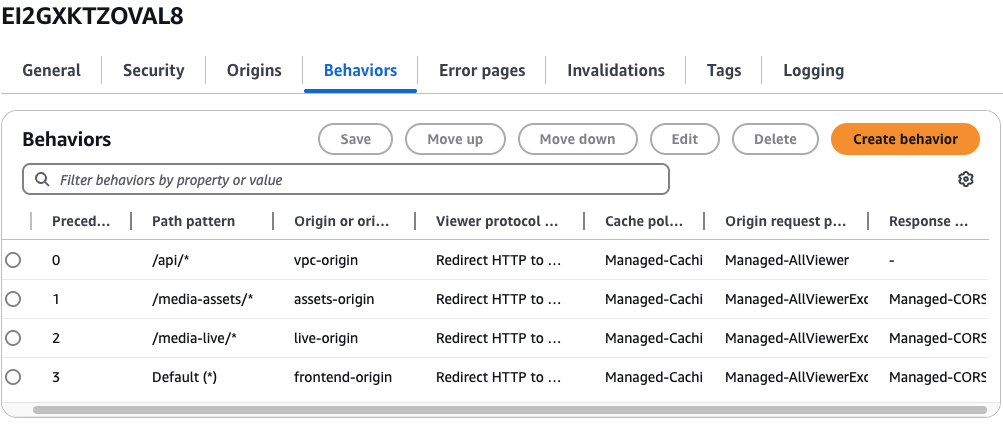
\includegraphics[width=150mm, keepaspectratio]{figures/distro_behav.png}
  \caption{Képernyőkép a különböző útvonalak cache szabályairól.}
  \label{fig:behav}
\end{figure}

A VPC Origin típusú origin a CloudFront-disztribúcióban egy Amazon VPC-n belüli erőforrást jelent -- a mi esetünkben ez az ALB-példányunk --, amelyet a CloudFront közvetlenül elérhet. Nem működik \emph{cross-account} módon, tehát amennyiben a célpont egy másik AWS-fiókban helyezkedne el. Az origin a VPC-n belül található, és elsősorban privát alhálózaton, Security Groupokkal van védve hálózati szinten. A~VPC Origin típusú origin használata lehetővé teszi, hogy a CloudFront közvetlenül kommunikáljon az erőforrással, anélkül hogy nyilvános doménnevet kelljen rendelni hozzá. Ezzel megspórolhatjuk az ALB-példány Internet Gateway-re való kötését, az ALB-példány számára domén bejegyzését, valamint SSL-tanúsítvány felvételét annak, a TLS-kapcsolat is terminálhat a CloudFront-disztribúcióban, házon belül már elég HTTP-alapon forgalmazni komponensek között.

\begin{figure}[h]
  \centering
  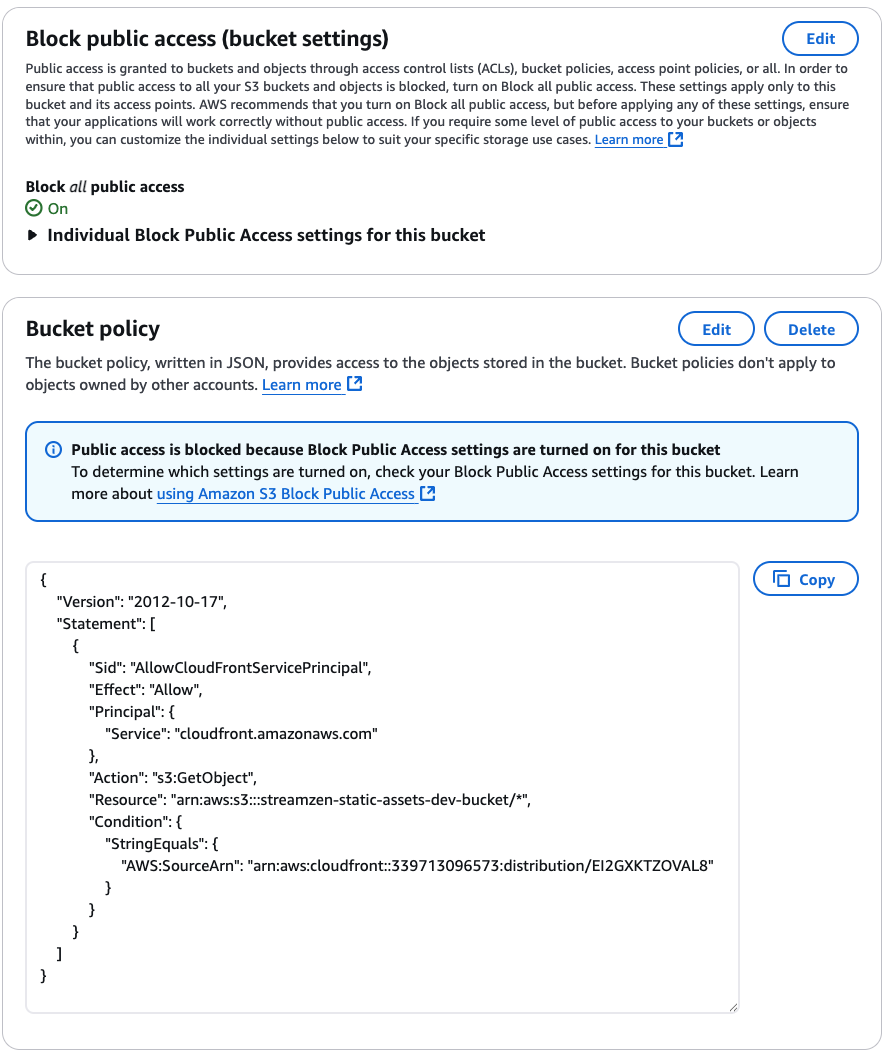
\includegraphics[width=130mm, keepaspectratio]{figures/distro_s3policy.png}
  \caption{Képernyőkép a vödrök hozzáférési beállításairól.}
  \label{fig:s3policy}
\end{figure}

Az S3-vödrök publikus elérését teljes blokkolásra állítottam (\refstruc{fig:s3policy}). Úgy tettem őket elérhetővé a CloudFront-disztribúció számára, hogy egy-egy ``bucket policy''-t csatoltam hozzájuk\cite{s3policy}, amely az S3 originre egyedi, arra csatolt Origin Access Controllal (OAC)\cite{oac} együtt lehetővé teszi, hogy csupán az az AWS-beli principal -- azaz a mi disztribúciónk -- kapjon az objektumolvasásokra (és csak arra) hozzáférést, amelynek a megadott Amazon Resource Number (ARN) azonosítója van. Az ábrán megadott \verb|AWS:SourceArn| a~\verb|streamzen-frontend-distro-dev| disztribúció ARN-je. A fent gyakorolt beállítás is biztosítja az IT-biztonságban is elterjedt és az AWS által is ösztönzött \emph{"principle of least privilege (PoLP)"} elvét.

\begin{figure}[h]
  \centering
  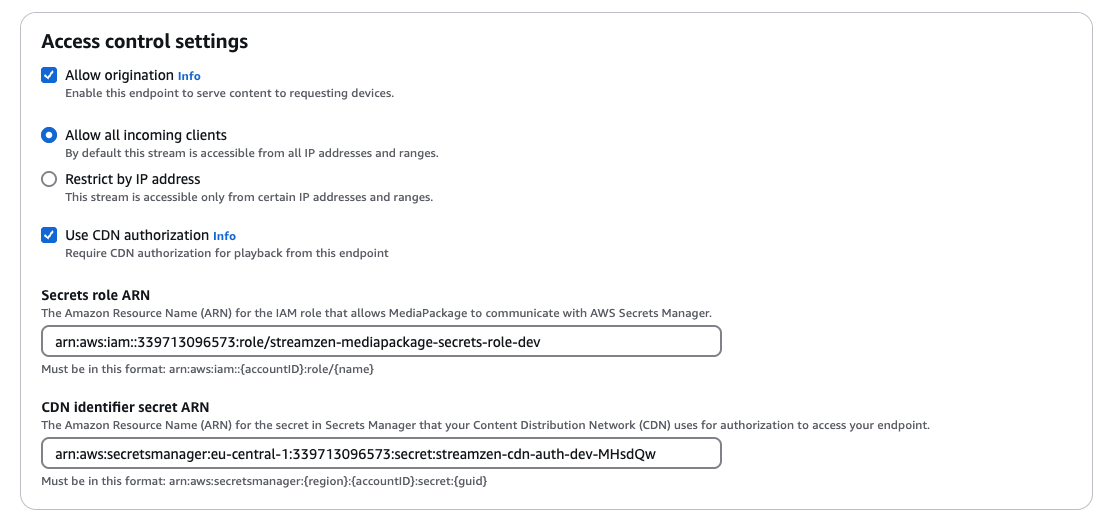
\includegraphics[width=150mm, keepaspectratio]{figures/distro_mediapack.png}
  \caption{Képernyőkép a HLS-végpont hozzáférési beállításairól.}
  \label{fig:mediapack}
\end{figure}

A MediaPackage-csatorna védettségét pedig a publikált HLS-végpontra beállított \emph{CDN Authorization}\cite{cdnauth} segítségével biztosítottam, amely a CloudFront-disztribúciótól érkező kérésekben a \verb|X-MediaPackage-CDNIdentifier| fejlécbe várja el egy titkos kulcs-érték párból az értéket. Ezt a fejlécet a disztribúció felkonfigurálásakor a megfelelő originra rátettem. A MediaPackage-csatorna HLS-végpontjának hozzáférési beállításait, a felhasznált Secret Managerből származó kulcs-érték pár ARN-jét, és az azt elérő IAM-szerep ARN-jét \az+\refstruc{fig:mediapack} mutatja be.

\section{A statikus weboldal}

A statikus weboldal HTML-, JavaScript- és CSS-fájlokból, valamint a weboldal statikus tartalmát képező médiafájlokból (képek, betűtípusok) tevődik össze. Ezek összeállításához a React keretrendszerben írt SPA-alkalmazásokat is jól kezelő Vite.js eszközt használtam, amely a React-alkalmazásokat egyetlen kiindulási \verb|index.html| HTML-fájlba csomagolja, és a készülő JavaScript-kódot is optimalizálja. A Vite.js a fejlesztési környezetben gyorsítótárazza a fájlokat, így gyorsabbá téve a fejlesztést, míg a gyártási környezetben (angolul \emph{in production}) optimalizálja azokat, hogy a lehető legkisebb méretűek legyenek.

Korábban bemutatásra került két különböző CloudFront Function-függvény, amelyek az S3-vödrök elérése előtt futnak minden kérésen. Ezek közül a statikus weboldal előtti függvény (\ref{lst:frontend}. kódrészlet) csupán arra hivatott, hogy a kéréseknél az egyes prefixekkel kezdődő kéréseket átirányítsa az alapértelmezett \verb|/| útvonalra. Ezekre azért volt szükség, hogy a statikus oldal által kezelt útvonalak mind a CDN-re való belépés után az alapértelmezett útvonalon elérhető \verb|index.html|-re oldódjanak fel, hiszen az indexoldalon behivatkozott JavaScriptből pedig majd a betöltés után a React Router megfelelően kezeli le a böngészőben az eredetileg kért útvonalat. Ez a megoldás természetesen magával vonzza azt az igényt, hogy akármikor, ha új aloldalt vezetünk be, akkor a CloudFront Function-függvényben ezt a prefixet hozzá kell adnunk a \verb|routingPrefixes| tömbhöz, amely a kód elején található.

\begin{minipage}{0.92\textwidth}
  \begin{lstlisting}[
  caption=frontend-request-default.js fájl tartalma.,
  label=lst:frontend,
  style=js,
  basicstyle=\fontsize{10}{12}\ttfamily
]
const routingPrefixes = ["/videos", "/live", "/events", "/members", "/courses", "/about", "/studio", "/login"];
function handler(event) {
  const request = event.request;
  if (routingPrefixes.some((pref) => request.uri.startsWith(pref))) {
    request.uri = "/";
  }
  return request;
}
\end{lstlisting}
\end{minipage}

A Vite.js ökoszisztémájának részét képzik különböző fejlesztők által összerakott kódgeneráló szkriptek, a Vite.js hivatalos dokumentációja által ajánlott szkriptek közül választottam a kezdőprojekt felállítására egy olyat, amely TypeScript nyelven írt és React keretrendszerre felkészítve rak össze egy kliensoldali NPM-projektet.

Ezek után telepítettem ebbe a projektbe a könnyebb fejlesztéshez szükséges könyvtárakat, ilyenek például a React Router, a React Hook Forms, az Axios és a Hls.js, utóbbi kettő jelentős szerepet fog még betölteni később implementációs kifejtéseimben. Ezek mellett UI-komponensek kódját húztam be a \emph{shadcn/ui}\footnote{\url{https://ui.shadcn.com/}} könyvtárából, amelyek a felhasználói felület megjelenítéséhez szükségesek.

A Vite.js képes fejlesztői módban indítani egy webszervert arra, hogy folyamatosan figyelje a fájlokat (úgynevezett \emph{watch mode}-ban), és ha változás történik, akkor újrabuildelje a fájlokat, és újraindítsa a webszervert.

\subsection{A weboldal telepítésének CI/CD-folyamata}\label{sec:ciCd}

Előkészítettem egy CI/CD-folyamatot \verb|lint-client.yml| néven a \verb|.github| mappa munkafolyamatai alatt, amely akkor fut le, ha a változtatások giten való feltöltése után készítünk egy Pull Requestet. Ez a munkafolyamat a következő lépéseket hajtja végre: statikus ellenőrzés ESLint\footnote{\url{https://eslint.org/}} használatával, kódformattálás ellenőrzése Prettier\footnote{\url{https://prettier.io/}} használatával, valamint a webalkalmazás lebuildelése. A három lépés hibátlan lefutása jelzi azt, hogy a változtatások után a webalkalmazás telepíthető lesz az S3-vödörbe.

Egy másik folyamat pedig a Pull Request elfogadása és a \verb|main| ágba való beolvasztása után indul el, amely a \verb|deploy-client.yml| néven található. \Az+\ref{lst:deployClient}. kódrészlet mutatja be a kódjának fontos részletét. Két \verb|job| jellemzi a folyamatot, amelyből a második, a konkrét telepítés függ az előző lefutásától, valamint kézzel kell elindítani, amint készen áll (ezt az \verb|environment: production| sor valósítja meg). Az elkészült teljes csomag a Node.js 20-as verziójával buildelődik, majd pedig az elkészült alkalmazás csomagja artifaktként kerül átadásra a következő jobnak. Letöltés után a telepítő szkript az AWS CLI segítségével a~megadott S3-vödörbe tölti fel a fájlokat. A \verb|aws| \verb|s3| \verb|sync| parancs használatával a fájlok feltöltése előtt törli a vödörből azokat a fájlokat, amelyek már nem találhatóak meg a~buildelt fájlok között, így biztosítva azt, hogy mindig csak a legfrissebb fájlok kerüljenek ki a vödörbe.

A GitHub Actionból való AWS-hez való hozzáférést egy külön kompozit akció valósítja meg (\verb|setup-aws| néven), amely az AWS által fenntartott hivatalos ``Configure AWS Credentials'' nevű GitHub Marketplace-en publikált akció\footnote{\url{https://github.com/marketplace/actions/configure-aws-credentials-action-for-github-actions}} v4-es verzióját használja. Ez az akció a megadott AWS IAM-szerepkörhöz tartozó hitelesítő adatokat állítja be a környezeti változókban, amelyeket a következő lépésben használhatunk.

A szerepkör, amelyet a környezet felvesz a \verb|github-oidc-pipeline| névre hallgat. Ezt a szerepkört az infra-bootstrap alprojektből telepítettem korábban az AWS-fiókba. A szerepkört úgy konfiguráltam be, hogy csupán a teljes projektet tároló \verb|streamzen-monorepo| nevű GitHub-repository számára adjon jogosultságot, azaz csak az innen futó GitHub Actionök tudják felvenni a szerepkört. Ez a szerepkör az, amelyet \ref{sec:config} alfejezet is a tervekben bemutatott, amely OIDC nyomán kap hozzáférést.

\begin{minipage}{0.92\textwidth}
  \begin{lstlisting}[
  caption=Részlet a deploy-client.yml fájl tartalmából.,
  label=lst:deployClient,
  style=yaml,
  basicstyle=\fontsize{10}{12}\ttfamily
]
build:
  runs-on: ubuntu-latest
  defaults:
    run:
      working-directory: client
  steps:
    - name: Checkout code
      uses: actions/checkout@v4
    - name: Setup Node.js
      uses: actions/setup-node@v4
      with:
        node-version: 20.x
    - name: Install dependencies
      run: corepack enable && yarn install
    - name: Build
      run: yarn build
    - name: Save bundle
      uses: actions/upload-artifact@v4
      with:
        name: bundle
        path: ./client/dist/
deploy:
  runs-on: ubuntu-latest
  needs: build
  environment: production
  steps:
    - name: Download bundle
      uses: actions/download-artifact@v4
      with:
        name: bundle
        path: /tmp/bundle/dist/
    - name: Setup AWS
      uses: ./.github/actions/setup-aws
    - name: Deploy
      run: aws s3 sync --delete /tmp/bundle/dist s3://streamzen-static-frontend-dev-bucket
\end{lstlisting}
\end{minipage}
